\documentclass[FM,DP]{tulthesis}

\usepackage[czech]{babel}
\usepackage[utf8]{inputenc}
\usepackage{graphicx}

\usepackage{listings}
\usepackage{color}

\TULtitle
{Online aplikace pro paralelní vykreslování webových stránek více renderovacími jádry \\a následnou obrazovou analýzou}
{Online applications for parallel rendering web pages rendering multiple cores \\and subsequent image analysis}
\TULprogramme{N2612}{Elektrotechnika a informatika}{Electrotechnology and informatics}
\TULbranch{1802T007}{Informační technologie}{Information technology}
\TULauthor{Bc. Jakub Jirouš}
\TULsupervisor{Ing. Mojmír Volf}
\TULyear{2017}

% Zobrazení Literatury v obsahu
\usepackage[nottoc]{tocbibind}

% Courier New font
\usepackage{courier}

\begin{document}

% Prohlášení
\ThesisStart{male}

% Abstrakt CZ
\begin{abstractCZ}
Český abstrakt

Klíčová slova

\end{abstractCZ}

\vspace{2cm}

% Abstrakt EN
\begin{abstractEN}
English abstract
\end{abstractEN}

\begin{acknowledgement}
Vám poděkování a lásku vám.
\end{acknowledgement}

% Obsah
\tableofcontents

% Seznam obrázků
\listoffigures

% Seznam tabulek
\listoftables

% Seznam zdrojových kódů
\renewcommand{\lstlistlistingname}{Seznam zdrojových kódů}
\renewcommand{\lstlistingname}{Zdrojový kód} % popisek u vložení zdrojového kódu
\lstlistoflistings

% definice barev pro vložení zdrojových kódů
\definecolor{codegreen}{RGB}{0,255,0}
\definecolor{codegray}{RGB}{169,183,198}
\definecolor{codeorange}{RGB}{178,80,39}
\definecolor{codeyellow}{RGB}{222,122,49}
\definecolor{codepurple}{RGB}{108,0,255}
\definecolor{codeblue}{RGB}{0,0,255}
\definecolor{backcolour}{RGB}{255,255,255}
 
 % definice stylu pro vložení zdrojových kódů
\lstdefinestyle{codestyle}{
    backgroundcolor=\color{backcolour},   
    commentstyle=\color{codegreen},
    keywordstyle=\color{codeyellow},
    numberstyle=\tiny\color{black},
    stringstyle=\color{codegreen},
    basicstyle=\ttfamily\footnotesize,
    breakatwhitespace=false,         
    breaklines=true,                 
    captionpos=b,        
    frame=single,
    keepspaces=true,                 
    numbers=left,                    
    numbersep=10pt,                  
    showspaces=false,                
    showstringspaces=false,
    showtabs=false,                  
    tabsize=1,
}

% aplikace stylu pro vložení zdrojových kódů
\lstset{style=codestyle}


% Seznam zkratek
\begin{abbrList}
\textbf{PHP} & Hypertext Preprocessor \\
\textbf{HTML} & HyperText Markup Language \\
\end{abbrList}



% ***[Hlavní text]*************************************************************************
\chapter{Úvod}

\section{Rešerše}

\section{Teoretická část}

\section{Praktická část}

\section{Rešerše}

\section{Rešerše}


\section{Vyhodnocení řešení}



\section{Shrnutí práce}



Screenshoty z aplikace

sdfsdfsddsf \cite{szeliski_2011} \cite{nixon_2012} \cite{parker_2011} \cite{tatroe_2013} \cite{FM_prirucka_Pliva}


\chapter{Testování Latex}


% block code
\begin{lstlisting}[language=php, caption=PHP example]
public function __construct(FormFactory $factory, SessionManager $sm, UserManager $um, UserRoleManager $rm)
{
  $this->factory = $factory;
  $this->sm = $sm;
  $this->um = $um;
  $this->rm = $rm;
}
\end{lstlisting}


\begin{lstlisting}[language=html, caption=HTML example]
<div class="alert alert-info" role="alert">
   There is no history yet.
</div>
\end{lstlisting}


\begin{lstlisting}[language=sql, caption=SQL example], label
SELECT * 
FROM 'shoot' 
ORDER BY 'date' DESC 
LIMIT 4
\end{lstlisting}


Řádek před seznamem.
\begin{itemize}
\item První položka.
\item Druhou uděláme delší,aby bylo vidět, jak ji\LaTeX\ bude formátovat. 

Může obsahovat několik odstavců.

\item Třetí položka.
\end{itemize}




\begin{enumerate}

\item První otázka.
\begin{enumerate}
\item buď
\item nebo \href{www.jakubjirous.cz}{odkaz}
\item anebo jinak
\end{enumerate}

\item Druhá otázka.
\begin{enumerate}
\item třeba
\item nebo ne
\item a co tohle?
\end{enumerate}

\end{enumerate}


\section{Podkapitola}

\subsection{PodPodkapitola}

\subsubsection{PodPodPodkapitola}

\paragraph{odstavec}

\subparagraph{pododstavec}


% Obrázek
% h - místě výskytu (here)
% t - na začátku stránky (top)
% b - na konci stránky (bottom)
% p - na samostatné stránce (page of ˿oats)
\begin{figure}[ht]
\centering
\includegraphics[scale=0.15]{images/text/01.jpg}
\caption{Test vložení obrázku}
\label{foto}
\end{figure}



% Seznam literatury
\renewcommand{\bibname}{Použitá literatura}
\bibliography{cites/bibliography}
\bibliographystyle{cites/czechiso}



% ***[Přílohy]*****************************************************************************
\appendix

% ***[Obsah CD]*******************************************************************************
\chapter{Obsah přiloženého CD}

\section{Text diplomové práce}
Adresář obsahuje veškerý text diplomové práce. 
\begin{itemize}
\item Desky\_diplomove\_prace\_2017\_Jakub\_Jirous.docx
\item Desky\_diplomove\_prace\_2017\_Jakub\_Jirous.pdf
\end{itemize}


\section{Použité obrázky v textu diplomové práce}
Adresář obsahuje obrázky použité v textové části diplomové práce.


\section{Zdrojové kódy aplikace}
V adresáři jsou obsaženy kompletní zdrojové kódy výsledné aplikace.


\section{Snímky obrazovky z výsledné aplikace}
Adresář obsahuje snímky z veškerých hlavních částí výsledné aplikace.


% ***[Snímky aplikace]************************************************************************
\chapter{Snímky obrazovky výsledné aplikace}

\section{Úvodní obrazovka}

% Obrázek
% h - místě výskytu (here)
% t - na začátku stránky (top)
% b - na konci stránky (bottom)
% p - na samostatné stránce (page of ˿oats)
\begin{figure}[h]
\centering
\includegraphics[scale=0.25]{images/screenshots/01.jpg}
\caption{Úvodní obrazovka}
\label{foto}
\end{figure}



\end{document}